\chapter{Neurale plasticiteit, leren en geheugen}\label{ch:b3:learning-memory}

In 1953 verwijderde een chirurg het binnenste deel van beide
slaapkwabben van een jongeman met onbehandelbare epilepsie. De
aanvallen namen af; de patiënt, vijftig jaar lang bekend als H.M.,
vormde nooit meer een blijvende herinnering aan een gebeurtenis. Hij
kon een gesprek voeren, leerde even goed als ieder ander een ster in
een spiegel na te tekenen --- en ontkende elke dag de taak ooit te
hebben gezien --- en hij herinnerde zich zijn jeugd. Het geheugen bleek
niet één ding te zijn, en het maken van nieuwe herinneringen aan
gebeurtenissen hing af van een structuur ter grootte van een duim. Wat
er in een brein verandert wanneer het leert is de oudste vraag van de
neurowetenschap, en het antwoord, uitgewerkt in een zeeslak met
twintigduizend neuronen en in coupes van de \omterm{def:b3:learning-memory:kinds}{hippocampus} van een rat,
luidt dat synapsen hun sterkte veranderen naar gelang wat er doorheen
gaat --- een regel die Donald Hebb in 1949 raadde en die een molecuul,
de \omterm{prop:b3:learning-memory:nmda}{NMDA-receptor}, bleek uit te voeren. Dit hoofdstuk behandelt die
regel en haar machinerie, de schakelingen die haar gebruiken om
plaatsen en gebeurtenissen op te slaan, de wiskunde die zegt wat zo'n
stelsel kan leren en hoeveel het kan bevatten, en het beloningssignaal
dat het vertelt wat de moeite van het leren waard is.

\section{Soorten geheugen en waar zij huizen}

\begin{definition}[Vormen van leren en geheugen]\label{def:b3:learning-memory:kinds}
\index{gewenning}\index{sensitisatie}\index{conditionering}\index{declaratief geheugen}\index{procedureel geheugen}\index{consolidatie}\index{hippocampus}
Het eenvoudigste leren is \emph{niet-associatief}: \emph{gewenning},
een afnemend antwoord op een herhaalde onschadelijke prikkel, en
\emph{sensitisatie}, een versterkt antwoord na een schadelijke.
\emph{Associatief} leren verbindt twee gebeurtenissen: bij
\emph{klassieke conditionering} (Pavlov) gaat een neutrale prikkel die
een beloning of een straf voorspelt het antwoord oproepen; bij
\emph{operante conditionering} wordt een handeling die wordt beloond
herhaald. Het menselijke geheugen valt uiteen in het
\emph{declaratieve} geheugen --- feiten en gebeurtenissen, bewust
opgeroepen, afhankelijk van de \emph{hippocampus} en de mediale
slaapkwab --- en het \emph{niet-declaratieve} geheugen ---
vaardigheden en gewoonten (striatum, \omterm{def:b3:nervous-systems:plan}{kleine hersenen}),
geconditioneerde angst (amygdala), priming (schors) --- dat in het
presteren tot uiting komt zonder herinnering. Een herinnering wordt
eerst in een labiele kortetermijnvorm vastgehouden, die seconden tot
uren duurt, en wordt in uren tot jaren \emph{geconsolideerd} tot een
stabiele langetermijnvorm die de hippocampus niet meer nodig heeft en
in de schors huist.
\end{definition}

\begin{proof}[Bewijsmateriaal]
Scoville en Milner (1957) beschreven H.M.: na verwijdering van beide
hippocampi en de aangrenzende schors waren zijn verstand en zijn
herinneringen van vóór de operatie grotendeels ongeschonden en was zijn
werkgeheugen normaal zolang hij zijn aandacht ergens op hield, maar hij
kon geen nieuwe herinnering aan enige gebeurtenis of enig feit vormen.
Hij leerde motorische vaardigheden in de loop van dagen in een normaal
tempo terwijl hij ontkende te hebben geoefend --- vaardigheidsgeheugen
had de \omterm{def:b3:learning-memory:kinds}{hippocampus} dus niet nodig --- en hij herinnerde zich het verre
verleden beter dan de jaren vlak voor de operatie, zodat de \omterm{def:b3:learning-memory:kinds}{hippocampus}
nodig was om declaratieve herinneringen vast te leggen en ze een tijd
lang vast te houden, maar niet om ze voorgoed te bewaren. Apen en
ratten met overeenkomstige laesies vertoonden dezelfde scheiding, en de
studie van één enkele patiënt heeft het vakgebied opnieuw ingericht.
\end{proof}

\section{De regel van Hebb en haar molecuul}

\begin{definition}[Hebbiaanse plasticiteit, LTP en LTD]\label{def:b3:learning-memory:ltp}
\index{regel van Hebb}\index{langetermijnpotentiëring}\index{langetermijndepressie}\index{pulstijdafhankelijke plasticiteit}
Hebb (1949) stelde voor dat wanneer een presynaptisch neuron
herhaaldelijk deelneemt aan het vuren van een postsynaptisch neuron, de
verbinding ertussen wordt versterkt --- ``cellen die samen vuren,
groeien samen''. \emph{Langetermijnpotentiëring} (LTP) is de
proefondervindelijke vorm daarvan: een korte reeks prikkels met hoge
frequentie op een baan laat de synapsen die zij activeerde urenlang
sterker achter in een coupe en wekenlang in een dier. LTP is
\emph{invoerspecifiek} (alleen de geprikkelde synapsen veranderen),
\emph{associatief} (een zwakke invoer die met een sterke naar dezelfde
cel wordt gepaard, wordt gepotentieerd) en vergt \emph{samenwerking}
tussen invoeren om de cel te depolariseren.
\emph{Langetermijndepressie} (LTD) is het omgekeerde, voortgebracht
door langdurige activiteit met lage frequentie. Bij
\emph{pulstijdafhankelijke plasticiteit} wordt het teken door de
volgorde bepaald: een presynaptische puls enkele milliseconden
\emph{vóór} de postsynaptische versterkt de synaps, een puls vlak
\emph{erna} verzwakt haar, binnen een venster van ongeveer
\qty{20}{ms} aan weerszijden --- zodat een synaps leert te voorspellen
en niet slechts samen te hangen.
\end{definition}

\begin{proposition}[De NMDA-receptor als gelijktijdigheidsmelder]\label{prop:b3:learning-memory:nmda}
\index{NMDA-receptor}\index{AMPA-receptor}\index{CaMKII}\index{CREB}\index{dendritische doorn}
Bij prikkelende synapsen werkt glutamaat op twee receptoren. De
\emph{AMPA}-receptor gaat open bij binding en draagt de gewone
synaptische stroom. De \emph{NMDA}-receptor bindt glutamaat maar wordt
bij de rustpotentiaal geblokkeerd door een magnesiumion in zijn porie;
alleen wanneer het postsynaptische membraan is gedepolariseerd --- door
vele invoeren tegelijk, of door een terugwaarts lopende
actiepotentiaal --- wordt het magnesium uitgedreven en geleidt het
kanaal, waarmee het calcium binnenlaat. De \omterm{prop:b3:learning-memory:nmda}{NMDA-receptor} gaat dus
alleen open wanneer de presynaptische afgifte (glutamaat) samenvalt met
postsynaptische activiteit (depolarisatie): hij is de ``en''-poort van
Hebb in één enkel eiwit. Het calcium dat een \emph{\omterm{prop:b3:learning-memory:nmda}{dendritische doorn}}
binnenkomt activeert het kinase \emph{CaMKII}, dat \omterm{prop:b3:learning-memory:nmda}{AMPA-receptoren}
fosforyleert en er meer van uit een voorraad de synaps in drijft --- de
synaps is binnen minuten sterker (vroege LTP). Een grote, trage
stijging van calcium activeert in plaats daarvan het fosfatase
calcineurine, dat \omterm{prop:b3:learning-memory:nmda}{AMPA-receptoren} weghaalt: LTD. Potentiëring die meer
dan enkele uren duurt (late LTP) vergt nieuw eiwit: kinasen bereiken de
kern, de transcriptiefactor \emph{CREB} zet genen aan, en de doorn
groeit en kan zich splitsen --- dezelfde eis van genexpressie die het
kortetermijngeheugen van het langetermijngeheugen scheidt in elk
bestudeerd dier.
\end{proposition}

\begin{proof}[Bewijsmateriaal]
Bliss en L\o mo (1973) prikkelden de perforante baan naar de
\omterm{def:b3:learning-memory:kinds}{hippocampus} van een konijn met een reeks pulsen en vonden het opgewekte
antwoord uren daarna nog vergroot --- de eerste LTP. Collingridge
(1983) toonde aan dat een blokker van de \omterm{prop:b3:learning-memory:nmda}{NMDA-receptor} (AP5) het
opwekken van LTP verhinderde maar het gewone synaptische antwoord niet;
Morris (1986) bracht AP5 in de \omterm{def:b3:learning-memory:kinds}{hippocampus} van ratten en vond dat zij
de plaats van een verborgen platform in een bassin met water niet meer
konden leren terwijl zij normaal zwommen en zagen; en muizen bij wie de
\omterm{prop:b3:learning-memory:nmda}{NMDA-receptor} alleen in het CA1-gebied van de \omterm{def:b3:learning-memory:kinds}{hippocampus} was
verwijderd misten daar zowel de LTP als het ruimtelijke geheugen.
Dezelfde receptor, op dezelfde plaats, was nodig voor de synaptische
verandering en voor het leren.
\end{proof}

\begin{omfigure}
\begin{tikzpicture}[every node/.style={font=\scriptsize}, >=stealth]
  % presynaptic terminal
  \draw[thick, omDef, fill=omDef!12] (0,2.2) .. controls (0,3.4) and (4,3.4) .. (4,2.2) -- (4,1.7) -- (0,1.7) -- cycle;
  \node at (2,2.8) {presynaptisch uiteinde};
  \foreach \p in {(0.8,2.0),(1.6,2.1),(2.6,2.0),(3.3,2.1)} \draw[thick, fill=omDef!40] \p circle (0.17);
  \foreach \p in {(1.2,1.45),(2.0,1.5),(2.9,1.42)} \fill[omProp] \p circle (0.06);
  \node[right, omProp] at (3.3,1.45) {glutamaat};
  % postsynaptic spine
  \draw[thick, omMeth!70!black, fill=omMeth!10] (-0.6,1.1) -- (4.4,1.1) -- (4.4,-1.2) -- (-0.6,-1.2) -- cycle;
  \node at (0.6,-0.9) {dendritische doorn};
  % AMPA
  \draw[thick, fill=omMeth!45] (0.2,0.85) rectangle (0.6,1.35); \node[below, align=center] at (0.1,0.8) {AMPA:\\Na$^{+}$ naar binnen};
  \draw[->, thick] (0.4,1.7) -- (0.4,0.95);
  % NMDA with Mg
  \draw[thick, fill=omThm!35] (2.4,0.85) rectangle (2.9,1.35); \fill[gray!70] (2.65,1.1) circle (0.09); \node[right, font=\tiny] at (2.95,1.1) {Mg$^{2+}$-blokkade};
  \node[below, align=center] at (2.65,0.8) {NMDA: vergt glutamaat\\\emph{én} depolarisatie};
  \draw[->, thick, omThm] (2.65,0.15) -- (2.65,-0.5) node[below] {Ca$^{2+}$};
  % downstream
  \node[draw, rounded corners, fill=omThm!15, font=\tiny] (cam) at (5.6,0.3) {CaMKII};
  \draw[->, thick] (2.9,-0.5) -- (cam);
  \node[draw, rounded corners, fill=omMeth!25, font=\tiny, align=center] (ampa) at (8.2,1.0) {meer AMPA-receptoren\\ingebracht: vroege LTP (minuten)};
  \node[draw, rounded corners, fill=omMeth!25, font=\tiny, align=center] (creb) at (8.2,-0.5) {CREB, nieuwe eiwitten,\\groei van de doorn: late LTP (uren+)};
  \draw[->, thick] (cam) -- (ampa.west); \draw[->, thick] (cam) -- (creb.west);
  \node[draw, rounded corners, fill=omDef!15, font=\tiny, align=center] (ltd) at (8.2,-1.8) {traag, klein Ca$^{2+}$: calcineurine,\\AMPA weggehaald: LTD};
  \draw[->, thick, dashed] (2.9,-0.7) .. controls (4.5,-1.6) .. (ltd.west);
\end{tikzpicture}

{\small De \omterm{prop:b3:learning-memory:nmda}{NMDA-receptor} als de poort van Hebb. Glutamaat alleen opent
\omterm{prop:b3:learning-memory:nmda}{AMPA-receptoren}; het NMDA-kanaal geleidt pas wanneer de doorn ook
gedepolariseerd is en zijn magnesium vertrekt. Het calcium dat dan
binnenkomt bepaalt de toekomst van de synaps: een snelle grote stijging
versterkt haar, een trage kleine verzwakt haar.}
\end{omfigure}

\begin{omfigure}
\begin{tikzpicture}
\begin{axis}[
  width=6.6cm, height=5.2cm,
  axis x line=bottom, axis y line=left,
  xmin=-20, xmax=120, ymin=0, ymax=220,
  xlabel={minuten}, ylabel={synaptisch antwoord (\%)},
  xlabel style={font=\small, at={(axis description cs:0.5,-0.12)}, anchor=north}, ylabel style={font=\small},
  tick label style={font=\scriptsize}, xtick={0,30,60,90,120}, ytick={0,100,200},
  clip=false,
]
\addplot[only marks, mark=*, mark size=1pt, omDef] coordinates {(-18,100) (-15,98) (-12,102) (-9,99) (-6,101) (-3,100) (2,195) (5,180) (8,172) (11,168) (15,165) (20,162) (30,160) (40,158) (50,157) (60,156) (70,156) (80,155) (90,155) (100,154) (110,154) (120,154)};
\addplot[only marks, mark=o, mark size=1pt, gray] coordinates {(-18,100) (-12,101) (-6,99) (2,102) (8,100) (15,101) (30,100) (45,99) (60,101) (75,100) (90,100) (105,101) (120,100)};
\draw[->, thick, omThm] (axis cs:0,215) -- (axis cs:0,200); \node[font=\scriptsize, omThm, anchor=south] at (axis cs:0,216) {tetanus};
\node[font=\scriptsize, omDef, anchor=south west] at (axis cs:35,168) {geprikkelde baan: LTP};
\node[font=\scriptsize, gray, anchor=north west] at (axis cs:35,95) {controlebaan: onveranderd};
\end{axis}
\begin{axis}[
  at={(7.6cm,0)}, anchor=south west,
  width=6.6cm, height=5.2cm,
  axis x line=middle, axis y line=middle,
  xmin=-60, xmax=60, ymin=-60, ymax=100,
  xlabel={$t_{\text{pre}} - t_{\text{post}}$ (ms)}, ylabel={$\Delta w$ (\%)},
  xlabel style={font=\small, at={(axis description cs:0.5,-0.06)}, anchor=north}, ylabel style={font=\small, at={(axis description cs:0.5,1.02)}, anchor=south},
  tick label style={font=\scriptsize}, xtick={-40,-20,20,40}, ytick={-40,40,80},
  clip=false,
]
\addplot[very thick, omMeth!70!black, domain=-60:-0.5, samples=60] {80*exp(x/15)};
\addplot[very thick, omThm, domain=0.5:60, samples=60] {-45*exp(-x/25)};
\node[font=\scriptsize, omMeth!70!black, anchor=south east] at (axis cs:-8,62) {pre vóór post: LTP};
\node[font=\scriptsize, omThm, anchor=north west] at (axis cs:8,-22) {post vóór pre: LTD};
\end{axis}
\end{tikzpicture}

{\small Links: \omterm{def:b3:learning-memory:ltp}{langetermijnpotentiëring} --- na een korte tetanus blijft
het antwoord van de geprikkelde baan urenlang vergroot terwijl een niet
geprikkelde baan naar dezelfde cellen onveranderd blijft
(invoerspecificiteit). Rechts: het venster van de pulstijd --- de
synaps versterkt als de presynaptische puls voorop loopt en verzwakt
als zij achterblijft.}
\end{omfigure}

\begin{theorem}[Wat een hebbiaanse synaps leert]\label{thm:b3:learning-memory:hebb}
\index{hebbiaans leren!hoofdcomponent}\index{regel van Oja}
Zij een neuron dat invoeren $\mathbf{x} = (x_{1},\dots,x_{n})$ ontvangt
via gewichten $\mathbf{w}$ en lineair antwoordt, $y = \mathbf{w}\cdot\mathbf{x}$.
De \omterm{def:b3:learning-memory:ltp}{regel van Hebb}, $\Delta\mathbf{w} = \eta\, y\,\mathbf{x}$, geeft
gemiddeld over de invoeren
\[
\langle\Delta\mathbf{w}\rangle = \eta\,C\,\mathbf{w}, \qquad C =
\langle\mathbf{x}\mathbf{x}^{\mathsf{T}}\rangle ,
\]
waarin $C$ de correlatiematrix van de invoeren is. De gewichten groeien
onbegrensd, en groeien het snelst langs de eigenvector van $C$ met de
grootste eigenwaarde: de synaps gaat het invoerpatroon waarnemen dat
het vaakst aanwezig is --- de \emph{hoofdcomponent} van haar invoeren.
Met een term die grote gewichten bestraft, de \emph{\omterm{thm:b3:learning-memory:hebb}{regel van Oja}}
$\Delta\mathbf{w} = \eta\, y\,(\mathbf{x} - y\,\mathbf{w})$, nadert de
gewichtsvector die eigenvector, genormeerd tot lengte één, en wordt het
neuron een stabiele melder van de overheersende correlatie in wat het
ziet.
\end{theorem}
\begin{proof}
Invullen van $y = \mathbf{w}\cdot\mathbf{x} = \mathbf{x}^{\mathsf{T}}
\mathbf{w}$ in de \omterm{def:b3:learning-memory:ltp}{regel van Hebb} geeft $\Delta\mathbf{w} = \eta\,\mathbf{x}
\mathbf{x}^{\mathsf{T}}\mathbf{w}$, waarvan het gemiddelde over de
invoeren (met een traag veranderende
$\mathbf{w}$) gelijk is aan $\eta C\mathbf{w}$. $C$ is symmetrisch en
positief semidefiniet, dus heeft zij loodrechte eigenvectoren $\mathbf{e}_{k}$
met eigenwaarden $\lambda_{k} \ge 0$; schrijft men $\mathbf{w} = \sum_{k}
a_{k}\mathbf{e}_{k}$, dan voldoet elke component aan $\Delta a_{k} = \eta\lambda_{k}
a_{k}$ en groeit zij als $(1 + \eta\lambda_{k})^{t}$, zodat de
component langs de grootste eigenwaarde de richting van $\mathbf{w}$
gaat overheersen terwijl de lengte divergeert. De \omterm{thm:b3:learning-memory:hebb}{regel van Oja} middelt
tot $\eta(C\mathbf{w} -
(\mathbf{w}^{\mathsf{T}}C\mathbf{w})\mathbf{w})$; in een vast punt geldt
$C\mathbf{w} = (\mathbf{w}^{\mathsf{T}}C\mathbf{w})\mathbf{w}$, dus is
$\mathbf{w}$ een eigenvector met $\lambda = \mathbf{w}^{\mathsf{T}}
C\mathbf{w} = \lambda|\mathbf{w}|^{2}$, en dus $|\mathbf{w}| = 1$; het
vaste punt langs de grootste eigenwaarde is het stabiele (een
verstoring naar een andere eigenvector krimpt, omdat de eigenwaarde
daarvan kleiner is), wat hier wordt aangenomen.
\end{proof}

\begin{example}[Twee invoeren]\label{ex:b3:learning-memory:two-inputs}
Een neuron ontvangt twee invoeren die gewoonlijk samen actief zijn, dus $C =
\begin{pmatrix} 1 & 0.8 \\ 0.8 & 1\end{pmatrix}$. De eigenvectoren zijn
$(1,1)/\sqrt{2}$ met eigenwaarde $1.8$ en $(1,-1)/\sqrt{2}$ met
eigenwaarde $0.2$. Uitgaande van $\mathbf{w} = (1, 0)$ draait de \omterm{def:b3:learning-memory:ltp}{regel
van Hebb} na vele kleine stappen $\mathbf{w}$ naar $(1,1)$: het neuron
leert op de twee invoeren \emph{samen} te antwoorden, en de zeldzame
gelegenheden waarop er maar één vuurt te negeren --- het heeft de
correlatie eruit gehaald. Met de \omterm{thm:b3:learning-memory:hebb}{regel van Oja} komen de gewichten uit
op $(0.71, 0.71)$. Dat is de zin waarin hebbiaanse synapsen leren wat
samengaat, en daarom volgt de associatieve eigenschap van LTP, het
paren van een zwakke invoer met een sterke, uit de regel.
\end{example}

\section{Een slak die leert}

\begin{proposition}[Sensitisatie bij \emph{Aplysia}]\label{prop:b3:learning-memory:aplysia}
\index{Aplysia}\index{presynaptische facilitatie}\index{cAMP}\index{PKA}
De zeeslak \emph{Aplysia} trekt haar kieuw terug wanneer haar sifon
wordt aangeraakt, een reflex van een paar dozijn herkenbare neuronen.
Een schok op de staart \emph{sensitiseert} haar: het terugtrekken bij
een lichte aanraking wordt versterkt, minuten lang na één schok en
weken lang na meerdere. Kandel en collega's (jaren 1970--1990)
herleidden de verandering tot de synaps tussen het sensorische neuron
van de sifon en het motorneuron van de kieuw. De schok op de staart
prikkelt een \omterm{def:b3:nervous-systems:cells}{interneuron} dat serotonine op het uiteinde van het
sensorische neuron afgeeft; serotonine verhoogt het cyclische AMP, dat
proteïnekinase A activeert, dat een kaliumkanaal fosforyleert en
sluit; de actiepotentialen van het uiteinde worden breder, er komt meer
calcium binnen en er wordt per puls meer overdrachtsstof afgegeven ---
\emph{\omterm{prop:b3:learning-memory:aplysia}{presynaptische facilitatie}}, een covalente verandering die
minuten duurt. Herhaalde schokken sturen het kinase naar de kern, waar
het CREB activeert, dat genen aanzet die nieuwe synaptische uiteinden
bouwen: het langetermijngeheugen bestaat uit meer synapsen, en het
wordt geblokkeerd door remmers van de eiwitsynthese die tijdens de
training worden gegeven maar niet erna. \emph{\omterm{def:b3:learning-memory:kinds}{Gewenning}} is het
omgekeerde, een verzwakking van dezelfde synaps; en \emph{klassieke
\omterm{def:b3:learning-memory:kinds}{conditionering}}, het paren van de aanraking met de schok, versterkt de
facilitatie bij de synapsen die vlak voor de aankomst van de serotonine
actief waren --- een hebbiaanse gelijktijdigheid die presynaptisch is
verwezenlijkt, door een adenylylcyclase dat door calcium en serotonine
samen wordt geprikkeld.
\end{proposition}

\begin{omfigure}
\begin{tikzpicture}[every node/.style={font=\scriptsize}, >=stealth]
  \node[draw, thick, rounded corners, fill=omDef!20, minimum width=2cm] (sn) at (0,0) {sensorisch neuron sifon};
  \node[draw, thick, rounded corners, fill=omMeth!25, minimum width=2cm] (mn) at (6.2,0) {motorneuron kieuw};
  \node[draw, thick, rounded corners, fill=omProp!30, align=center] (in) at (2.8,2.4) {faciliterend interneuron\\(serotonine)};
  \node[left] at (-2.1,0) {aanraking}; \draw[->, thick] (-2.0,0) -- (sn);
  \draw[->, very thick] (sn) -- (mn) node[pos=0.45, below, align=center, font=\tiny] {de synaps\\die verandert};
  \draw[->, thick] (mn) -- (8.4,0) node[right] {kieuw trekt terug};
  \node[above] at (2.8,3.1) {schok op de staart}; \draw[->, thick] (2.8,3.05) -- (in);
  \draw[->, thick, omProp] (in) -- (2.8,0.25);
  \node[right, align=left, font=\tiny] at (6.6,1.6) {serotonine $\to$ cAMP $\to$ PKA\\$\to$ K$^{+}$-kanaal gesloten\\$\to$ bredere puls, meer Ca$^{2+}$,\\meer overdrachtsstof (minuten)\\herhaald: PKA $\to$ CREB\\$\to$ nieuwe uiteinden (weken)};
\end{tikzpicture}

{\small De schakeling van de \omterm{def:b3:learning-memory:kinds}{sensitisatie} bij \emph{Aplysia}.
Serotonine uit een \omterm{def:b3:nervous-systems:cells}{interneuron} werkt op het sensorische uiteinde, en
dezelfde synaps draagt het kortetermijngeheugen als een gefosforyleerd
kanaal en het langetermijngeheugen als nieuwe uiteinden.}
\end{omfigure}

\begin{omfigure}
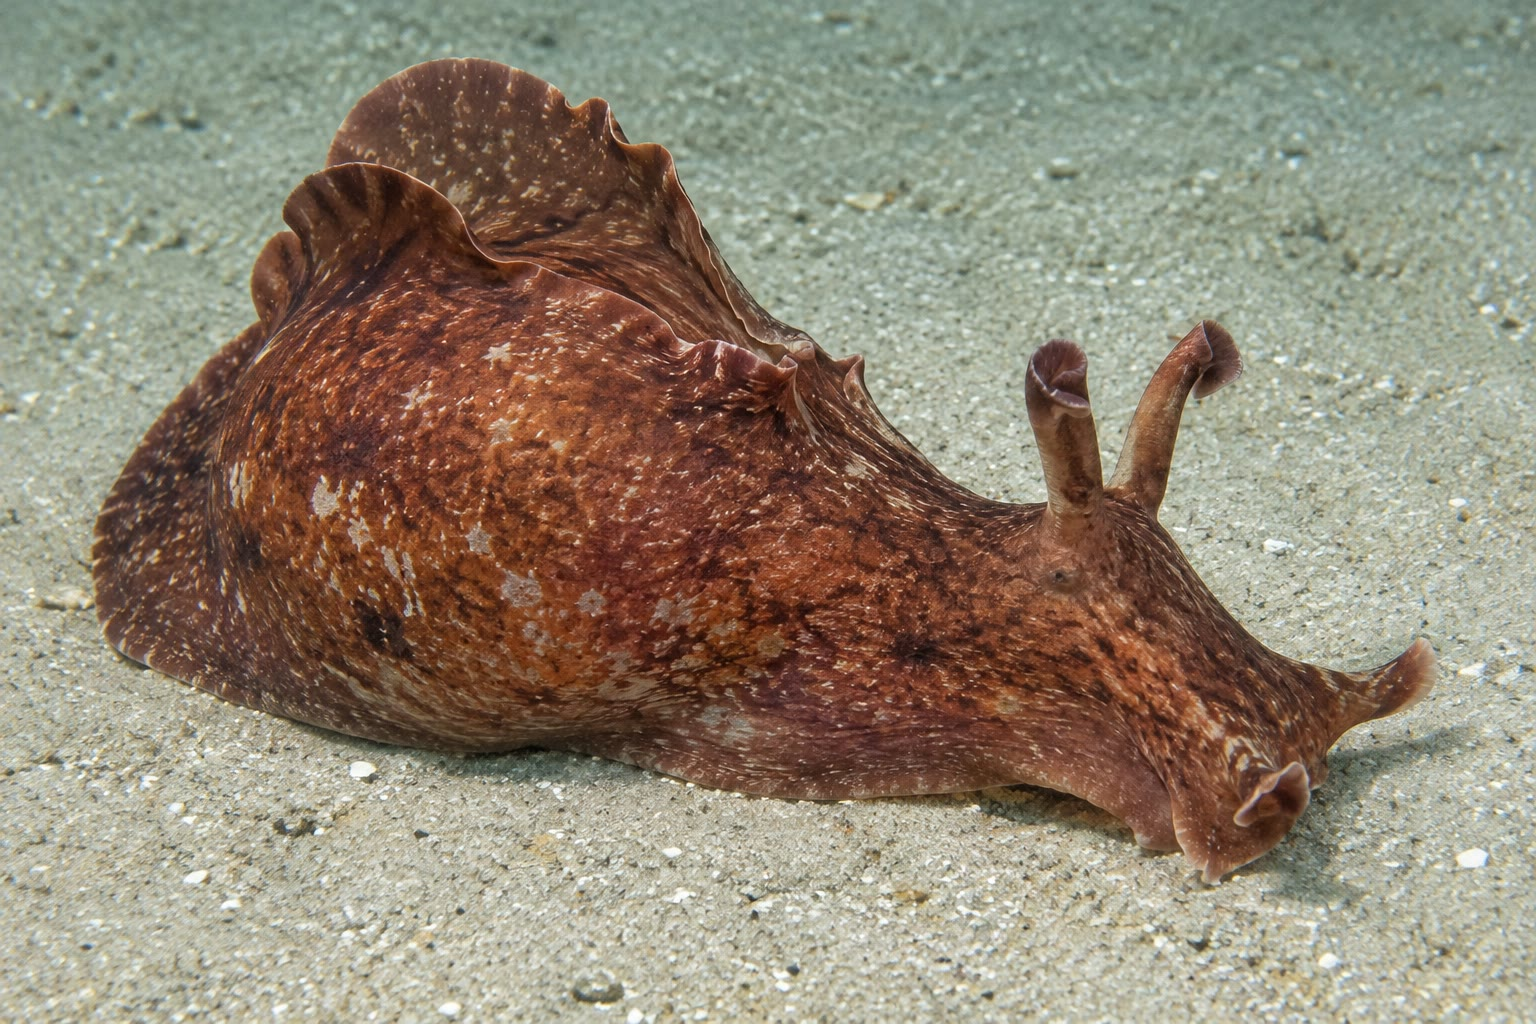
\includegraphics[width=0.46\linewidth]{images/book5/ai/b5-19-aplysia.jpg}\hspace{0.04\linewidth}
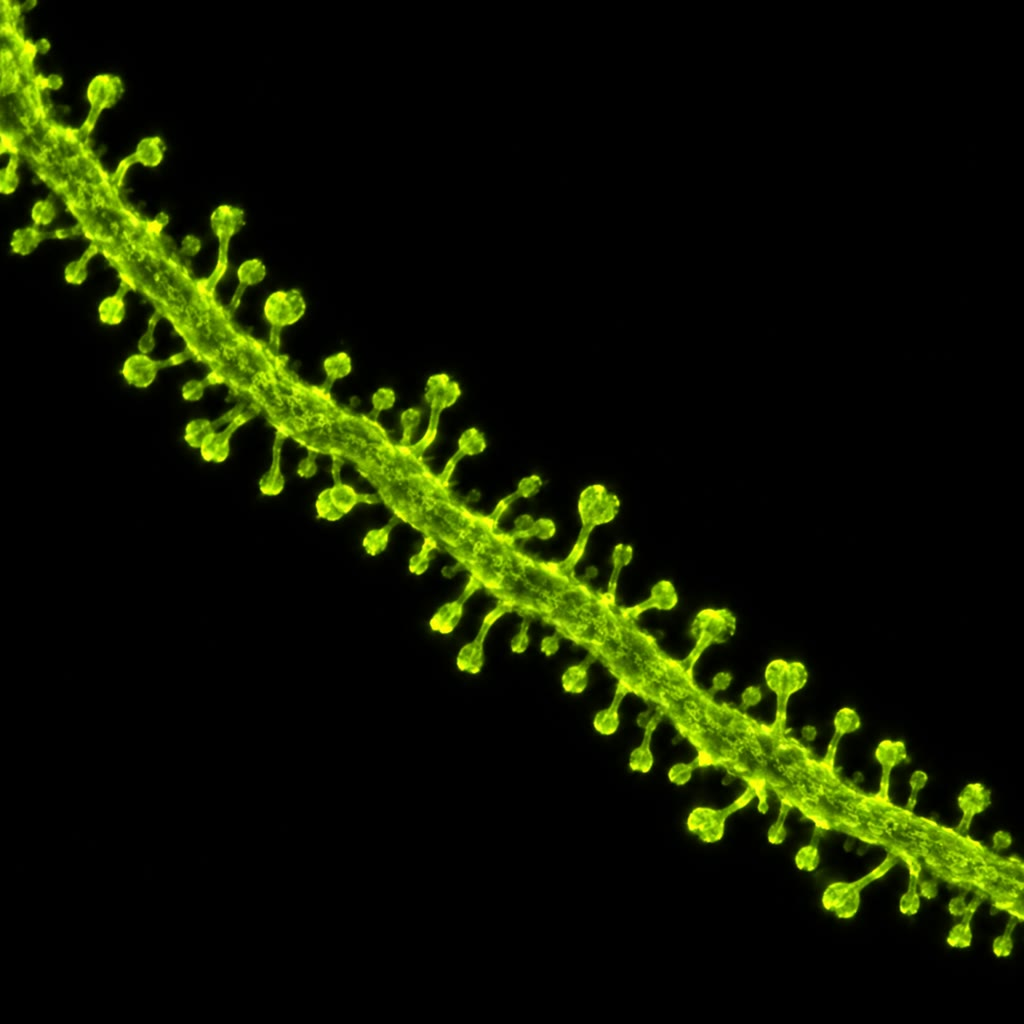
\includegraphics[width=0.36\linewidth]{images/book5/ai/b5-19-dendritic-spines.jpg}

{\small Links: \emph{Aplysia californica}, wier weinige en grote
neuronen het mogelijk maken de synaps van een herinnering te vinden en
te meten. Rechts: een dendriet bezaaid met doornen, elk de
postsynaptische zijde van één prikkelende synaps en elk een
compartiment waarvan het calcium het eigen lot beslist.}
\end{omfigure}

\section{Schakelingen voor plaatsen en gebeurtenissen}

\begin{definition}[De schakeling van de hippocampus]\label{def:b3:learning-memory:hippocampus}
\index{gyrus dentatus}\index{CA3}\index{CA1}\index{plaatscel}\index{roostercel}\index{patroonaanvulling}\index{herafspelen}
De invoer uit de schors bereikt de \omterm{def:b3:learning-memory:kinds}{hippocampus} via de entorhinale
schors en doorloopt drie trappen: de \emph{gyrus dentatus}, wier
korrelcellen talrijker zijn dan hun invoeren en spaarzaam vuren
(waarmee zij gelijkende patronen scheiden); \emph{CA3}, wier
piramidecellen onderling terugkerend zijn verbonden en elk duizenden
synapsen van andere ontvangen --- een \emph{auto-associatief} netwerk
dat een opgeslagen patroon uit een fragment kan aanvullen; en
\emph{CA1}, die de uitvoer van CA3 met de rechtstreekse invoer
vergelijkt en het resultaat aan de schors teruggeeft. Bij een rat die
een arena verkent vuurt een piramidecel van de \omterm{def:b3:learning-memory:kinds}{hippocampus} alleen
wanneer het dier zich op één plaats bevindt --- een \emph{plaatscel}
(O'Keefe, 1971) --- en enkele honderden ervan brengen de arena in
kaart; stroomopwaarts, in de entorhinale schors, vuren
\emph{roostercellen} (Moser, 2005) op de hoekpunten van een zeshoekig
rooster dat de ruimte bedekt, een coördinatenstelsel waaruit de
plaatsvelden worden opgebouwd. Tijdens de slaap en de rust worden de
reeksen plaatscellen die tijdens een tocht hebben gevuurd op hoge
snelheid \emph{herafgespeeld}, en het blokkeren daarvan schaadt de
herinnering aan de tocht: de \omterm{def:b3:learning-memory:kinds}{hippocampus} repeteert de paden van de dag
voor de schors.
\end{definition}

\begin{omfigure}
\begin{tikzpicture}[every node/.style={font=\scriptsize}, >=stealth]
  % trisynaptic loop
  \node[draw, thick, rounded corners, fill=gray!15, align=center] (ec) at (0,0) {entorhinale schors\\(roostercellen)};
  \node[draw, thick, rounded corners, fill=omDef!20, align=center] (dg) at (3.2,1.4) {gyrus dentatus:\\patroonscheiding};
  \node[draw, thick, rounded corners, fill=omProp!30, align=center] (ca3) at (7.2,1.4) {CA3, terugkerend:\\patroonaanvulling};
  \node[draw, thick, rounded corners, fill=omMeth!25, align=center] (ca1) at (7.2,-1.4) {CA1:\\vergelijkt, geeft uit};
  \draw[->, thick] (ec) -- (dg); \draw[->, thick] (dg) -- (ca3); \draw[->, thick] (ca3) -- (ca1); \draw[->, thick] (ca1) -- (ec) node[pos=0.3, below, sloped, font=\tiny] {terug naar de schors};
  \draw[->, thick, dashed] (ec) -- (ca1.north west) node[pos=0.7, above, sloped, font=\tiny] {rechtstreekse weg};
  \draw[->, thick, omProp!80!black] (ca3.north) .. controls (6.6,2.6) and (7.8,2.6) .. (ca3.north east) node[pos=0.5, above, font=\tiny] {terugkerende zijtakken};
  % place field map
  \begin{scope}[xshift=10.4cm, yshift=-0.2cm]
    \draw[thick] (0,0) rectangle (3,2.4); \node[below] at (1.5,-0.05) {arena, van bovenaf gezien};
    \foreach \p/\c in {(0.7,1.8)/omThm, (2.1,1.9)/omDef, (1.4,0.9)/omMeth, (2.5,0.6)/omProp} { \fill[\c!60] \p circle (0.32); \fill[\c!90] \p circle (0.16); }
    \node[above] at (1.5,2.45) {de vuurvelden van vier plaatscellen};
  \end{scope}
\end{tikzpicture}

{\small Links: de lus van de \omterm{def:b3:learning-memory:kinds}{hippocampus} --- scheiding in de \omterm{def:b3:learning-memory:hippocampus}{gyrus
dentatus}, opslag en aanvulling in het terugkerende \omterm{def:b3:learning-memory:hippocampus}{CA3}, vergelijking in
\omterm{def:b3:learning-memory:hippocampus}{CA1}. Rechts: elke \omterm{def:b3:learning-memory:hippocampus}{plaatscel} vuurt in één gebied van een arena; samen
brengen zij de ruimte in kaart.}
\end{omfigure}

\begin{proposition}[Hoeveel een auto-associatief netwerk bevat]\label{prop:b3:learning-memory:capacity}
\index{Hopfield-netwerk}\index{geheugencapaciteit}
Een netwerk van $N$ neuronen, elk met alle andere verbonden met
hebbiaanse gewichten $w_{ij} \propto \sum_{\mu}\xi_{i}^{\mu}\xi_{j}^{\mu}$
gesommeerd over de opgeslagen binaire patronen $\xi^{\mu}$, haalt een
opgeslagen patroon uit een aangetaste of onvolledige aanwijzing terug
door erin te bezinken als in een attractor (Hopfield, 1982). Dat lukt
betrouwbaar tot ongeveer $P
\approx 0.14N$ willekeurige patronen; daarboven storen de patronen
elkaar en stort het terughalen in. Het \omterm{def:b3:learning-memory:hippocampus}{CA3} van een rat, met zo'n
$3\times 10^{5}$ piramidecellen, zou naar deze schatting zo'n
$4\times 10^{4}$ patronen kunnen bevatten --- de orde van het aantal
verschillende plaatsen of episoden dat een dier in een seizoen
tegenkomt --- en het spaarzame vuren (enkele procenten van de cellen
actief in enig patroon) verhoogt de capaciteit nog. \omterm{def:b3:learning-memory:hippocampus}{Patroonaanvulling}
uit een aanwijzing is wat een geur of een hoek een heel tafereel laat
oproepen; de prijs is dat gelijkende herinneringen samenvloeien, wat de
scheiding door de \omterm{def:b3:learning-memory:hippocampus}{gyrus dentatus} tegengaat.
\end{proposition}
\admitted

\begin{method}[Geheugen en zijn mechanisme toetsen]\label{met:b3:learning-memory:tests}
\index{waterdoolhof van Morris}\index{angstconditionering}\index{engram}
(1) Een ruimtelijke taak: het \omterm{met:b3:learning-memory:tests}{waterdoolhof van Morris} --- een rat zwemt
in ondoorzichtig water naar een platform dat op een vaste plaats
verborgen ligt, leert de positie ervan in de loop van dagen uit de
aanwijzingen in de kamer, en wordt getoetst aan de tijd die hij in het
juiste kwadrant zoekt wanneer het platform is weggehaald; laesies van
de \omterm{def:b3:learning-memory:kinds}{hippocampus}, blokkers van NMDA en het verlies van LTP heffen het
leren elk op. (2) Een associatieve taak: angstconditionering --- een
toon die met een schok aan de poot wordt gepaard gaat verstijven
oproepen; de herinnering hangt af van de amygdala, en een versie die aan
de omgeving is gebonden van de \omterm{def:b3:learning-memory:kinds}{hippocampus}. (3) Een toets van het
mechanisme: blokkeer de kandidaat (een geneesmiddel, een uitschakeling
beperkt tot één gebied en één tijdstip) en laat zien dat het leren
mislukt terwijl de waarneming en de beweging dat niet doen. (4) Het
engram: merk de neuronen die tijdens het leren actief zijn met een
lichtgevoelig kanaal (\cref{ch:b3:nervous-systems}) en activeer ze
later opnieuw met licht --- het dier verstijft in een veilige omgeving,
alsof het zich herinnert; het stilleggen ervan blokkeert het oproepen.
Het geheugen zit in aanwijsbare cellen en hun synapsen, en kan worden
aan- en uitgezet.
\end{method}

\begin{omfigure}
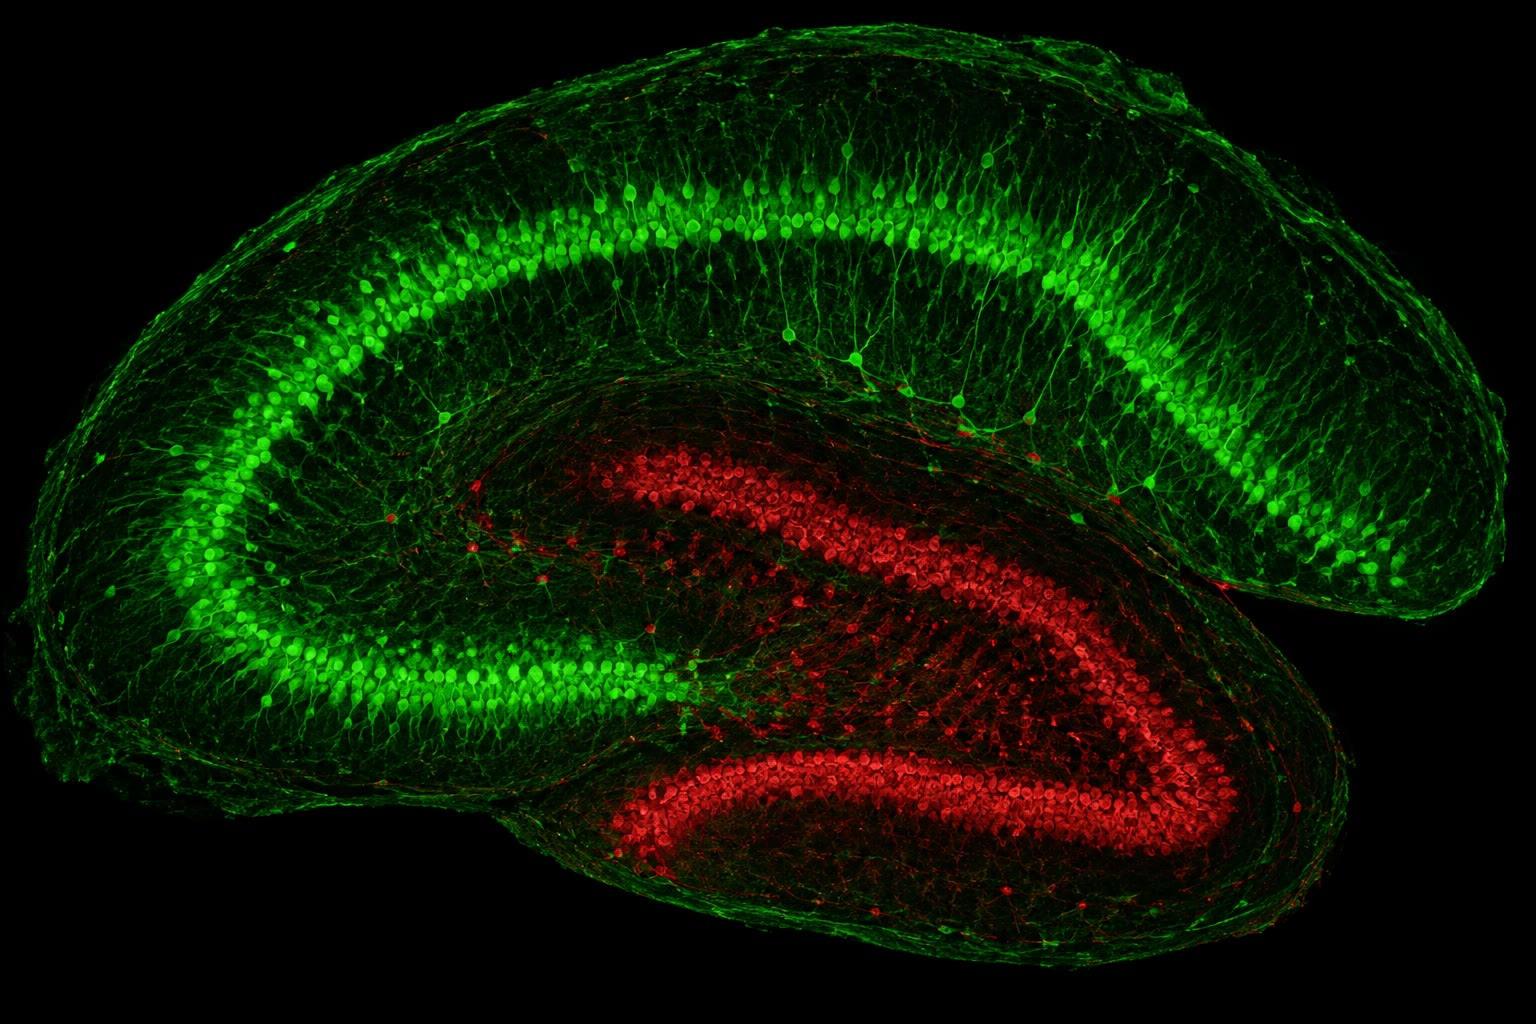
\includegraphics[width=0.56\linewidth]{images/book5/ai/b5-19-hippocampus-section.jpg}

{\small Een doorsnede door de \omterm{def:b3:learning-memory:kinds}{hippocampus} van een knaagdier: de gebogen
band piramidecellen (groen) van \omterm{def:b3:learning-memory:hippocampus}{CA3} naar \omterm{def:b3:learning-memory:hippocampus}{CA1} en de daarin grijpende
\omterm{def:b3:learning-memory:hippocampus}{gyrus dentatus} (rood). Elke ruimtelijke herinnering van het dier gaat
door deze lus.}
\end{omfigure}

\section{Beloning, voorspelling en de plasticiteit van een leven}

\begin{proposition}[Leren uit de voorspellingsfout]\label{prop:b3:learning-memory:rescorla}
\index{regel van Rescorla--Wagner}\index{voorspellingsfout}\index{dopamine}
Zij $V$ de waarde die een dier aan een aanwijzing hecht en $\lambda$ de
beloning die erop volgt. De \omterm{prop:b3:learning-memory:rescorla}{regel van Rescorla--Wagner} (1972) zegt dat
de waarde bij elke poging verandert met een deel $\alpha$ van de
\emph{voorspellingsfout}:
\[
\Delta V = \alpha\,(\lambda - V), \qquad
V_{n} = \lambda\bigl(1 - (1-\alpha)^{n}\bigr) ,
\]
zodat het leren eerst snel gaat en vertraagt naarmate de voorspelling
beter wordt, stopt zodra de beloning volledig is voorspeld, en omkeert
(uitdoving) wanneer de beloning wordt onthouden. Worden twee
aanwijzingen samen aangeboden, dan delen zij één voorspelling, zodat
een aanwijzing die niets toevoegt aan een reeds gemaakte voorspelling
niet wordt geleerd (\emph{blokkering}). Schultz (1997) mat de
dopamineneuronen van de middenhersenen bij apen en vond dat zij vuren
bij een onverwachte beloning, zwijgen bij een volledig voorspelde, en
onder hun rustniveau duiken wanneer een voorspelde beloning uitblijft:
zij zenden $\lambda - V$, de voorspellingsfout zelf, uit naar het
striatum en de schors, waar dopamine de plasticiteit vrijgeeft bij de
synapsen die kort tevoren actief waren. Leren wat een beloning
voorspelt is hebbiaanse plasticiteit met een derde factor die zegt of
de uitkomst beter of slechter was dan verwacht --- en verslavende
middelen, die de dopamine rechtstreeks aandrijven, vervalsen een
blijvend ``beter dan verwacht''.
\end{proposition}
\begin{proof}
De recursie $V_{n+1} = V_{n} + \alpha(\lambda - V_{n})$ geeft
$\lambda - V_{n+1} = (1-\alpha)(\lambda - V_{n})$, dus krimpt de fout
meetkundig, $\lambda - V_{n} = (1-\alpha)^{n}\lambda$ vanaf $V_{0} =
0$, waaruit de formule volgt. Voor twee aanwijzingen $A$ en $B$ die
samen worden aangeboden is de voorspelling $V_{A} + V_{B}$; is $A$
eerst tot $V_{A} = \lambda$ getraind, dan is de fout bij de
samengestelde pogingen nul en verwerft $B$ niets.
\end{proof}

\begin{omfigure}
\begin{tikzpicture}
\begin{axis}[
  width=6.6cm, height=5.0cm,
  axis x line=bottom, axis y line=left,
  xmin=0, xmax=25, ymin=0, ymax=1.1,
  xlabel={poging $n$}, ylabel={$V_{n}/\lambda$},
  xlabel style={font=\small, at={(axis description cs:0.5,-0.14)}, anchor=north}, ylabel style={font=\small},
  tick label style={font=\scriptsize}, xtick={0,5,10,15,20,25}, ytick={0,0.5,1},
  clip=false,
]
\addplot[very thick, omDef, domain=0:12, samples=13] {1-0.8^x};
\addplot[very thick, omDef, domain=12:25, samples=14] {(1-0.8^12)*0.8^(x-12)};
\draw[dashed, gray] (axis cs:12,0) -- (axis cs:12,1.05);
\node[font=\scriptsize, anchor=north west, align=left] at (axis cs:0.5,0.98) {beloning gegeven:\\verwerving};
\node[font=\scriptsize, anchor=north west, align=left] at (axis cs:14,0.98) {beloning onthouden:\\uitdoving};
\end{axis}
\begin{axis}[
  at={(7.6cm,0)}, anchor=south west,
  width=6.6cm, height=5.0cm,
  ybar, bar width=14pt,
  axis x line=bottom, axis y line=left,
  ymin=-1.2, ymax=1.5,
  symbolic x coords={onverwachte beloning, voorspelde beloning, beloning uitgebleven},
  xtick=data, ytick={-1,0,1}, yticklabels={duik,rustniveau,salvo},
  ylabel={vuren van dopamine},
  x tick label style={font=\scriptsize, align=center, text width=1.9cm}, ylabel style={font=\small}, tick label style={font=\scriptsize},
  clip=false,
]
\addplot[fill=omThm!50, draw=omThm] coordinates {(onverwachte beloning,1.2) (voorspelde beloning,0.05) (beloning uitgebleven,-1.0)};
\end{axis}
\end{tikzpicture}

{\small Links: de leerkromme van Rescorla--Wagner met $\alpha = 0.2$
--- een meetkundige nadering van de waarde van de beloning, daarna
uitdoving wanneer de beloning stopt. Rechts: dopamineneuronen melden de
voorspellingsfout --- een salvo bij een verrassing, niets bij een
voorspelde beloning, een duik wanneer een voorspelde beloning
uitblijft.}
\end{omfigure}

\begin{definition}[Kritieke perioden en de ziekten van de plasticiteit]\label{def:b3:learning-memory:critical}
\index{kritieke periode}\index{oogdominantie}\index{verslaving}\index{ziekte van Alzheimer}
De plasticiteit is het grootst in vensters van de ontwikkeling. Hubel
en Wiesel (jaren 1960) bedekten één oog van een kitten gedurende enkele
weken na de geboorte: de visuele schors, die normaal door beide ogen in
afwisselende kolommen wordt aangedreven, werd bijna geheel door het
open oog aangedreven, en het beroofde oog bleef levenslang functioneel
blind --- terwijl dezelfde beroving bij een volwassen kat niets
veranderde. Zulke \emph{kritieke perioden}, voor het zien, voor de
taal, voor de zang van vogels, sluiten wanneer de remmende
schakelingen rijpen en de extracellulaire matrix verstijft, en zij
laten zich met geneesmiddelen en training een weinig heropenen. De
pathologieën van de plasticiteit zijn een kwestie van dosis en doel:
\emph{verslaving} is leren dat door een vervalste voorspellingsfout
wordt gedreven en gewoonten bouwt die het genot overleven;
posttraumatische stress is een angstherinnering die door stresshormonen
te sterk is geconsolideerd; en de \emph{ziekte van Alzheimer} begint
waar het declaratieve geheugen begint, in de entorhinale schors en de
\omterm{def:b3:learning-memory:kinds}{hippocampus}, met het verlies van synapsen --- dat de dementie beter
volgt dan enige telling van plaques --- vóór het verlies van neuronen.
\end{definition}

\begin{remark}[Waaruit het geheugen bestaat]\label{rem:b3:learning-memory:what}
Een herinnering is geen opname maar een verandering in de sterkten en
de aantallen van synapsen, verdeeld over de cellen die actief waren
toen zij werd gemaakt, vastgelegd door een regel die versterkt wat
samen vuurt, vrijgegeven door een signaal dat zegt of de uitkomst
ertoe deed, en in de slaap gerepeteerd tot de schors haar zelf
vasthoudt. De regel is die van Hebb, de poort is de \omterm{prop:b3:learning-memory:nmda}{NMDA-receptor}, het
signaal is dopamine, de repetitie is het \omterm{def:b3:learning-memory:hippocampus}{herafspelen}, en de wiskunde
zegt wat zo'n stelsel kan bevatten en waarom het het gelijkende
verwart. Elk experiment dat een herinnering heeft aan- of uitgezet ---
met een blokker, een gen, een lichtstraal --- heeft haar in die
synapsen en in die cellen gevonden. H.M. stierf in 2008; zijn brein, in
coupes gesneden en afgebeeld, toonde de laesie die het vakgebied had
onderwezen, en niets meer.
\end{remark}

\section{Opgaven}

\begin{exercise}[$\star$]\label{exo:b3:learning-memory:1}
Onderscheid het declaratieve van het niet-declaratieve geheugen aan de
hand van de prestaties van H.M., en noem voor elk van vier soorten
niet-declaratief geheugen een hersengebied.
\end{exercise}

\begin{exercise}[$\star$]\label{exo:b3:learning-memory:2}
Formuleer het postulaat van Hebb en de drie eigenschappen van LTP die
eruit volgen.
\end{exercise}

\begin{exercise}[$\star$]\label{exo:b3:learning-memory:3}
Leg uit waarom de \omterm{prop:b3:learning-memory:nmda}{NMDA-receptor} een gelijktijdigheidsmelder is, en wat
er met LTP gebeurt wanneer zijn blokker AP5 vóór en wanneer hij ná de
tetanus wordt toegediend.
\end{exercise}

\begin{exercise}[$\star$]\label{exo:b3:learning-memory:4}
Wat onderscheidt bij \emph{Aplysia} de kortdurende van de langdurige
\omterm{def:b3:learning-memory:kinds}{sensitisatie} op moleculair niveau, en welk experiment laat dat zien?
\end{exercise}

\begin{exercise}[$\star\star$]\label{exo:b3:learning-memory:5}
Hoeveel pogingen zijn er bij $\alpha = 0.3$ nodig tot $V$ \qty{90}{\%}
van $\lambda$ bereikt? Als de beloning daarna wordt onthouden, hoeveel
pogingen tot $V$ onder \qty{10}{\%} zakt? Waarom zijn verwerving en
uitdoving in dit model symmetrisch, en zijn zij dat bij dieren?
\end{exercise}

\begin{exercise}[$\star\star$]\label{exo:b3:learning-memory:6}
Twee invoeren hebben $C = \begin{pmatrix}1 & 0.5\\ 0.5 & 1\end{pmatrix}$.
Bepaal de eigenvectoren en eigenwaarden, en zeg naar welke richting de
\omterm{def:b3:learning-memory:ltp}{regel van Hebb} de gewichten draait en wat het neuron dan waarneemt. Pas
de \omterm{thm:b3:learning-memory:hebb}{regel van Oja} één stap toe vanaf $\mathbf{w} = (1,0)$ met invoer $\mathbf{x}
= (1,1)$ en $\eta = 0.1$.
\end{exercise}

\begin{exercise}[$\star\star$]\label{exo:b3:learning-memory:7}
Een doorn heeft een volume van \qty{0.1}{fL}. Het binnenkomen van $500$
calciumionen verhoogt de vrije concentratie erin met hoeveel (in
$\unit{\micro mol/L}$), als \qty{95}{\%} onmiddellijk door buffers
wordt gebonden? Vergelijk met de rustwaarde van
\qty{0.1}{\micro mol/L} en met de $K_{d}$ van calmoduline, de activator
van CaMKII, ongeveer \qty{1}{\micro mol/L}.
\end{exercise}

\begin{exercise}[$\star\star$]\label{exo:b3:learning-memory:8}
Verklaar de blokkering met de \omterm{prop:b3:learning-memory:rescorla}{regel van Rescorla--Wagner} en geef voor
elke fase de bijbehorende meting aan de dopamineneuronen.
\end{exercise}

\begin{exercise}[$\star\star$]\label{exo:b3:learning-memory:9}
Voorspel de uitkomst van (a) verwijdering van de \omterm{prop:b3:learning-memory:nmda}{NMDA-receptor} beperkt
tot \omterm{def:b3:learning-memory:hippocampus}{CA1}, (b) een remmer van de eiwitsynthese tijdens de training
gegeven, (c) dezelfde remmer een dag later gegeven, (d) optogenetische
heractivering, in een nieuwe omgeving, van de cellen van de \omterm{def:b3:learning-memory:hippocampus}{gyrus
dentatus} die tijdens een angstconditionering actief waren.
\end{exercise}

\begin{exercise}[$\star\star\star$]\label{exo:b3:learning-memory:10}
Laat zien dat onder de \omterm{def:b3:learning-memory:ltp}{regel van Hebb} alleen de lengte van
$\mathbf{w}$ onbegrensd groeit, en dat de \omterm{thm:b3:learning-memory:hebb}{regel van Oja} in elk vast
punt $|\mathbf{w}| = 1$ geeft. Waarom is onbegrensde groei biologisch
een probleem, en welke mechanismen (synaptische schaling, LTD, slaap)
zouden met de normerende term kunnen overeenkomen?
\end{exercise}

\begin{exercise}[$\star\star\star$]\label{exo:b3:learning-memory:11}
Het \omterm{def:b3:learning-memory:hippocampus}{CA3} van een rat heeft $3\times 10^{5}$ cellen, dat van een mens
ongeveer $2\times 10^{6}$. Schat de capaciteit van Hopfield van elk.
Waarom is die schatting een slechte maat voor het aantal herinneringen
dat een mens bewaart, en wat voegt de rol van de \omterm{def:b3:learning-memory:kinds}{hippocampus} bij de
\omterm{def:b3:learning-memory:kinds}{consolidatie} aan het beeld toe?
\end{exercise}

\begin{exercise}[$\star\star\star$]\label{exo:b3:learning-memory:12}
Kittens die weken lang het zicht in één oog missen verliezen het gebied
van de schors van dat oog; volwassen dieren niet. Verklaar met
hebbiaanse mededinging waarom het open oog wint, waarom beroving van
beide ogen minder effect heeft dan van één, en wat de \omterm{def:b3:learning-memory:critical}{kritieke periode}
afsluit.
\end{exercise}

\section{Vraagstuk: een synaps die onthoudt}

\begin{problem}[{Weekendvraagstuk --- een herinnering gevolgd van het
calcium in een doorn tot een rat in een doolhof: de calciumrekenkunde
van de opwekking, een hebbiaans neuron dat convergeert naar wat zijn
invoeren delen, een leerkromme geklokt door de voorspellingsfout, en de
capaciteit van een hippocampus, eindigend bij de calciumconcentratie
die LTP opwekt, het aantal pogingen dat een rat nodig heeft en de
patronen die zijn CA3 kan bevatten}]
\label{pb:b3:learning-memory:1}
Gegevens: een doorn met een volume van \qty{0.08}{fL}; elk NMDA-kanaal
draagt $10^{3}$ Ca$^{2+}$ per opening van \qty{50}{ms}; een synaps
heeft $10$ \omterm{prop:b3:learning-memory:nmda}{NMDA-receptoren}; \qty{98}{\%} van het binnenkomende calcium
wordt gebufferd; vrij calcium in rust \qty{0.1}{\micro mol/L}; CaMKII
wordt geactiveerd boven \qty{2}{\micro mol/L} vrij calcium,
calcineurine tussen $0.3$ en
\qty{1}{\micro mol/L}. Hebb: twee invoeren met $C = \begin{pmatrix}1 &
0.6\\ 0.6 & 1\end{pmatrix}$, $\eta = 0.1$. Rescorla--Wagner: $\alpha =
0.15$. Capaciteit: \omterm{def:b3:learning-memory:hippocampus}{CA3} van een rat $3\times 10^{5}$ cellen,
$P = 0.14N$; een rat verkent $20$ nieuwe plaatsen per dag.

\medskip
\noindent\textbf{Deel I --- Calcium.}
\begin{enumerate}
  \item Alle tien \omterm{prop:b3:learning-memory:nmda}{NMDA-receptoren} gaan eenmaal open. Hoeveel
        calciumionen komen er binnen, hoeveel blijven er vrij, en welke
        stijging van de concentratie is dat in de doorn?
  \item Wordt CaMKII geactiveerd? En als er maar twee receptoren
        opengaan (glutamaat afgegeven maar de doorn nauwelijks
        gedepolariseerd)?
  \item Welk enzym bevindt zich met twee open receptoren in zijn
        bereik, en wat gebeurt er met de synaps? Leg uit hoe één ion
        zowel LTP als LTD kan voortbrengen.
  \item Calcium wordt met een tijdconstante van \qty{20}{ms}
        weggepompt. Waarom moeten invoeren binnen tientallen
        milliseconden aankomen om hun calcium op te tellen, en hoe legt
        dit het venster van de pulstijd vast?
  \item Een doorn ligt \qty{0.5}{\micro m} van zijn buur op de
        dendriet. Leg uit waarom de buffering en de nauwe hals van de
        doorn het calciumsignaal in één doorn houden, en waarom dat van
        belang is voor de invoerspecificiteit.
  \item De blokkade door magnesium wordt bij ongeveer \qty{-30}{mV}
        opgeheven. Eén AMPA-synaps depolariseert de doorn met
        \qty{5}{mV} vanaf \qty{-70}{mV}. Hoeveel gelijktijdige invoeren
        (of wat anders) zijn er nodig om \omterm{prop:b3:learning-memory:nmda}{NMDA-receptoren} te
        deblokkeren? Wat zegt dit over de samenwerking?
\end{enumerate}

\medskip
\noindent\textbf{Deel II --- Een hebbiaans neuron.}
\begin{enumerate}[resume]
  \item Bepaal de eigenwaarden en eigenvectoren van $C$.
  \item Pas vanaf $\mathbf{w} = (1, 0)$ de gemiddelde \omterm{def:b3:learning-memory:ltp}{regel van Hebb}
        $\mathbf{w} \leftarrow \mathbf{w} + \eta C\mathbf{w}$ drie
        stappen toe. Wat is na elke stap de hoek van $\mathbf{w}$ met
        de richting $(1,1)$?
  \item Wat is na vele stappen de verhouding $w_{2}/w_{1}$, en wat
        gebeurt er met $|\mathbf{w}|$?
  \item Pas de gemiddelde \omterm{thm:b3:learning-memory:hebb}{regel van Oja} $\mathbf{w} \leftarrow \mathbf{w} +
        \eta\,(C\mathbf{w} - (\mathbf{w}^{\mathsf{T}}C\mathbf{w})
        \mathbf{w})$ één stap toe vanaf $(0.8, 0.8)$. Waarheen beweegt
        zij?
  \item Het neuron antwoordt nu op de twee invoeren samen. Als invoer 2
        alleen vuurt (zeldzaam), wat is dan $y$ ten opzichte van het
        gezamenlijke geval, met $\mathbf{w} = (0.71, 0.71)$?
  \item Leg in één zin uit hoe de associativiteit van LTP (een zwakke
        invoer die met een sterke wordt gepaard, wordt versterkt) deze
        stelling in werking is.
\end{enumerate}

\medskip
\noindent\textbf{Deel III --- Leerkromme.}
\begin{enumerate}[resume]
  \item Bereken met $\alpha = 0.15$ de waarde van $V_{n}/\lambda$ na
        $5$, $10$ en $20$ pogingen.
  \item Hoeveel pogingen zijn er nodig om \qty{95}{\%} van $\lambda$ te bereiken?
  \item Een rat leert een doolhof in ongeveer dat aantal pogingen.
        Voorspelt het model sneller leren in pogingen als de beloning
        wordt verdubbeld? Wat verandert er?
  \item Aanwijzing A wordt tot de asymptoot getraind, daarna worden A
        en B $20$ pogingen lang samen met dezelfde beloning aangeboden.
        Wat is $V_{B}$? Wat doen de dopamineneuronen bij de
        samengestelde pogingen?
  \item De beloning volgt nu op B alleen. Beschrijf de
        voorspellingsfout en het dopamine-antwoord bij de eerste
        poging, en het verloop van $V_{B}$.
  \item Een geneesmiddel verhoogt de dopamine ongeacht de uitkomst. Leg
        met de regel uit waarom de handelingen die aan het middel
        voorafgaan worden geleerd alsof zij werden beloond, wat de
        gevolgen ervan ook zijn.
\end{enumerate}

\medskip
\noindent\textbf{Deel IV --- De \omterm{def:b3:learning-memory:kinds}{hippocampus}.}
\begin{enumerate}[resume]
  \item De capaciteit van Hopfield van het \omterm{def:b3:learning-memory:hippocampus}{CA3} van de rat.
  \item Hoe lang duurt het bij $20$ nieuwe plaatsen per dag voordat de
        capaciteit is bereikt? Wat moet er gebeuren opdat het dier kan
        blijven leren?
  \item De \omterm{def:b3:learning-memory:kinds}{consolidatie} draagt herinneringen in de loop van weken over
        aan de schors. Leg uit waarom een trage overdracht oude
        herinneringen in de schors beschermt (catastrofale storing) en
        waarom de \omterm{def:b3:learning-memory:kinds}{hippocampus} een tijdelijke opslag is.
  \item Als \qty{3}{\%} van de CA3-cellen in enig patroon actief is,
        hoeveel cellen coderen dan één plaats, en hoeveel patronen
        zouden er te onderscheiden zijn als patronen minder dan de
        helft van hun cellen mochten delen? (Beredeneer in grote lijnen
        waarom spaarzame codering de capaciteit verhoogt.)
  \item Het \omterm{def:b3:learning-memory:hippocampus}{herafspelen} tijdens de slaap perst een tocht van
        \qty{10}{s} samen tot \qty{0.5}{s}. Welke afstand tussen het
        vuren van plaatscellen in de tocht wordt bij een venster van de
        pulstijd van \qty{20}{ms} hebbiaans in het \omterm{def:b3:learning-memory:hippocampus}{herafspelen}? Waarom
        zou dat het nut van de samenpersing kunnen zijn?
  \item De herinnering aan het doolhof overleeft een laesie van de
        \omterm{def:b3:learning-memory:kinds}{hippocampus} die een maand na de training wordt gemaakt, maar
        niet een die een dag erna wordt gemaakt. Leg dat uit, met het
        verliespatroon van H.M.
  \item Vat samen: de concentratie vrij calcium na tien NMDA-openingen
        (vraag~1), het aantal pogingen tot \qty{95}{\%} leren
        (vraag~14), en de capaciteit van het \omterm{def:b3:learning-memory:hippocampus}{CA3} van de rat (vraag~19).
\end{enumerate}
\end{problem}
